\def\difficulty{1}
\sujet{Local Binary Patterns}\index{Features!Local Binary Patterns}
\begin{note}This tutorial aims to study a texture descriptor named 'Local Binary Patterns'. The first objective is to implement this descriptor. Therefater, digital images of textures will be classified using this descriptor and the k-means algorithm.  
\end{note}

\noindent The different processes will be applied on this kind of texture images:
{
	\makeatletter
	\renewcommand\fs@ruled{\def\@fs@cfont{\bfseries}\let\@fs@capt\floatc@ruled
		\def\@fs@pre{\hrule height.8pt depth0pt \kern2pt}%
		\def\@fs@post{\kern2pt\hrule\relax}%
		\def\@fs@mid{\vskip2pt}%
		\let\@fs@iftopcapt\iftrue}
	\makeatother
\begin{figure}[H]
\centering
\subfloat[metal image]{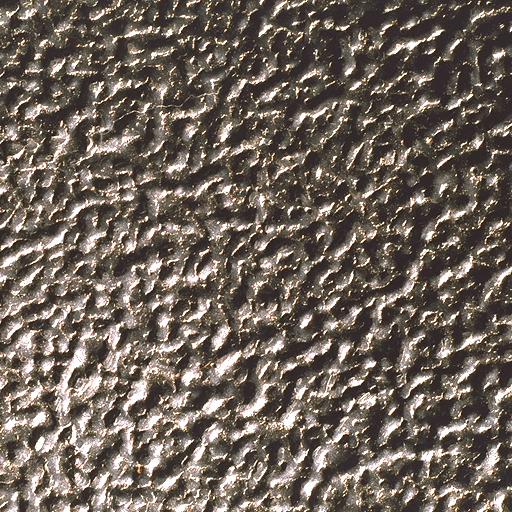
\includegraphics[width=.3\linewidth]{Metal1}}
\hfill
\subfloat[sand image]{
\includegraphics[width=.3\linewidth]{Sand1}}
\hfill
\subfloat[ground image]{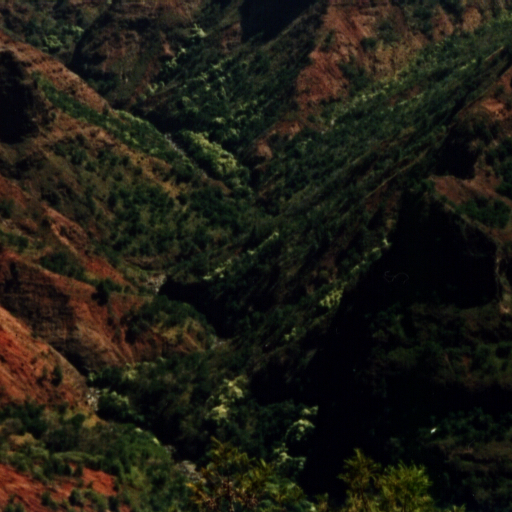
\includegraphics[width=.3\linewidth]{Terrain1}}
\vspace*{-5pt}
\end{figure}
}
%
\section{Local Binary Patterns}
The Local Binary Patterns (LBP) descriptor is a simple yet very efficient texture operator which labels the pixels of an image by thresholding the neighborhood of each pixel and considers the result as a binary number. Due to its discriminative power and computational simplicity, LBP texture operator has become a popular approach in various applications. It can be seen as a unifying approach to the traditionally divergent statistical and structural models of texture analysis. Perhaps the most important property of the LBP operator in real-world applications is its robustness to monotonic gray-scale changes caused, for example, by illumination variations. Another important property is its computational simplicity, which makes it possible to analyze images in challenging real-time settings.\\
The LBP feature vector, in its simplest form, is created in the following manner:
\begin{itemize}
\item For each pixel, compare the pixel to each of its 8 neighbors (on its left-top, left-middle, left-bottom, right-top, etc.). Follow the pixels along a circle, i.e. clockwise or counter-clockwise.
\item Where the center pixel's value is greater than the neighbor's value, write "1". Otherwise, write "0". This gives an 8-digit binary number (which is usually converted to decimal for convenience).
\item Compute the histogram of the frequency of each "number" occurring (i.e., each combination of which pixels are smaller and which are greater than the center).
\item Normalize the histogram.
\end{itemize}

\begin{figure}[h]
\centering
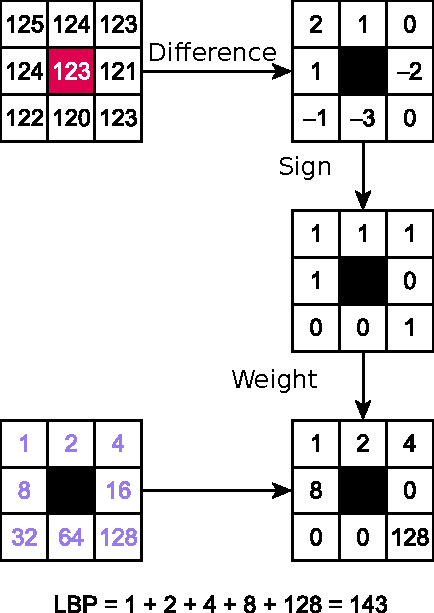
\includegraphics[width=.4\linewidth]{Lbp_computation.pdf}

\caption{Local binary pattern. From wikipedia, author Xiawi, CC-By-SA.}
\end{figure}
\begin{qbox}
\begin{itemize}
\item
Code a function for computing the Local Binary Patterns.
\item Test this operator on a texture image from the given database.
\end{itemize}
\end{qbox}

\begin{mcomment}
\begin{mremark}
Consider the function \minline{hiscounts} for histogram computation.
\end{mremark}
\end{mcomment}

\begin{pcomment}
\begin{premark}
Consider the function \minline{numpy.histogram} for histogram computation.
\end{premark}
\end{pcomment}


\section{Classification of texture images}
\index{Classification}
\index{Segmentation!K-means}
The objective is to classify the texture images from the given databse by using the LBP descriptor.
\begin{qbox}
\begin{enumerate}
\item Calculate the LBP descriptor for each image of the database.
\item Compare the descriptors for each class of images. 
\item Compute the distance between each pair of images in order to get a dissimilarity matrix. Comment the result.
\item Use the k-means algorithm to classify the images of the database into three classes ($k=3$). 
\end{enumerate}
\end{qbox}

\begin{mcomment}
\begin{mremark}
See \minline{kmeans}.
\end{mremark}
\end{mcomment}

\begin{pcomment}
\begin{premark}
See  \pinline{KMeans} from \pinline{sklearn.cluster}.
\end{premark}
\end{pcomment}
